\chapter{Instrumentation} % Write in your own chapter title
\label{chap:ins}
\lhead{Chapter 2. \emph{Instrumentation}} % Write in your own chapter title to set the page header

In Chap.~\ref{chap:ins} it was explained with detail the emission of AGN and its classification, derived from a great variety of spectral energy distributions. This fact makes the selection of an unbiased, uniform and complete sample of AGN an extremely difficult task. In order to perform a proper selection of active galaxies it is needed to understand the limits of each wavelength range.  

AGN were in first place detected at radio frequencies being called them Quasi Stellar Radio sources (and after, Quasars or QSO), but only a small fraction of objects emits strongly in the radio band. In the optical band it is where the maximum of emission of the AGN is, optical surveys provide large samples of AGN, but the selection techniques dramatically misses reddened objects and even host galaxy dominated ones. Infrared selection techniques are the most efficient ones to detect sources that are highly obscured and missed in the rest of the spectral bands, but this works for high luminosity sources, as it is needed to distinguish between the host IR emission and the contribution from the dust heated from the AGN.

In this thesis we used an X-ray selection based on the 2-10 keV energies. This band is sensible to X-ray absorption up to the Compton Thick limit (\NH $\sim$10$^{24}$ cm$^{-2}$). This AGN are found in the X-rays surveys identifying the counterparts in the optical for the X-ray sources, by cross-correlation of catalogs or by dedicated observations of the sources.

The selection used in this thesis is from the wide-angle (44.43 sq. degree) Bright Ultra-hard XMM-Newton Survey \citep{mateos12}. This is a flux limited ($f_{\rm 4.5-10\,keV}\geq$ 6$\times 10^{-14}$ erg s$^{-1}$ cm$^{-2}$) hard X-ray selected (4.5-10 keV) sample using the XMM-Newton observatory. The BUXS survey and the sample used are described in detail in Chap.~\ref{chap:buxs}.

This chapter will explain the instrumentation used to detect the active galaxies in the X-rays using XMM-Newton in Sec.~\ref{sec2:xr} and in the optical in Sec.~\ref{sec2:tel}, and more precisely using long-slit spectra form dedicated observations (Sec.~\ref{sec2:otel}) and fiber spectra from public surveys (Sec.~\ref{sec2:sdss}).

\section{X-ray observations}
\label{sec2:xr}

The atmosphere of the Earth is completely opaque to photons of certain energy as seen in Fig.~\ref{sec2:atm}. For some of the wavelength bands, the detectors must be at a certain altitude in order to detect its radiation. Optical emission can be detected from instruments located at the ground, as well fro some infrared energy windows. But in order to collect data from X-ray emission it is needed to place detectors in rockets or space observatories. 

 \begin{figure}
 \centering
 \includegraphics[width=\textwidth]{Chapter2_data/opac.ps}
 \includegraphics[width=\textwidth]{Chapter2_data/trans.ps}
    \caption{Top: Opacity of the atmosphere in terms of the observed wavelength (credit: NASA). Bottom: Altitude in kilometers in order to observe each wavelength range (credit: Thomson Higher Education 2007). }
 \label{sec2:atm}
 \end{figure}
 
In this thesis the X-ray data that is used comes from the X-ray Multi-Mirror satellite XMM-Newton. This is one of the four 'Cornerstone' missions defined in the Horizon 2000 Programme of the European Space Agency (ESA). 


 %\includegraphics[width=10cm]{Chapter2_data/opac.ps}




\subsection{XMM-Newton}
\label{sec2:xmm}

The spacecraft XMM-Newton was launched by an Ariane 504 from Kourou, French Guiana on 10 December 1999. The satellite is orbiting in a elliptical orbit around the Earth, with an inclination of 40$^{o}$, being the apogee at a distance between 99000 and 115000 km and the perigee between 6000 and 22000 km of altitude. The spacecraft takes 48 hours to complete an orbit.

The observatory XMM-Newton carries three scientific instruments, that are the European Photon Imaging Camera (EPIC;  \citealt{turner01}, \citealt{struder01}, see Sec.~\ref{sec2:epic}) the Reflection Grating Spectrometer (RGS; \citealt{denherder01}, see Sec.~\ref{sec2:rgs}) and the Optical Monitor telescope (OM; \citealt{mason01}, see Sec.~\ref{sec2:om}) that allows simultaneous optical and X-ray observations. In Fig.~\ref{sec2:xmmsch} we show a sketch of the XMM-Newton spacecraft.

 \begin{figure}
 \centering
 \includegraphics[width=\textwidth]{Chapter2_data/xmm.ps}
    \caption{Diagram of the XMM-Newton spacecraft (credit: ESA).}
 \label{sec2:xmmsch}
 \end{figure}
 

The three X-rays telescopes are build with 58 Wolter I grazing-incidence mirrors, being the largest mirrors of 70 cm of diameter. They are nested in coaxial and cofocal configuration with a grazing angle of 30'. The focal length of these telescopes is 7.5 m. This configuration allows that the instruments can achieve a an effective area of $\sim$ 1500 cm$^{2}$ over a wide energy range (0.1-15 keV), in particular at energies close to the rest frame Fe K$\alpha$ line.


\subsubsection{European Photon Imaging Camera (EPIC)}
\label{sec2:epic}


The European Photon Imaging Camera (EPIC) are Charge-Coupled Device cameras (CCD) that can register extremely weak X-ray radiation and can detect flux variation in the range of microseconds. these advanced Charge-Coupled Device cameras (CCD) are capable of detecting rapid variations in intensity in the range of $\sim$0.001 seconds.


They are located at the prime focus of each of the three telescopes. The EPIC camera have the following detectors, two Metal Oxide Semi-conductor (EPIC-MOS; \citealt{turner01}) and one EPIC-pn \citep{struder01}. In front of the detector, it is located a filter wheel.

\begin{itemize}

\item The EPIC-MOS consists on two sets of CCDs sensible in the 0.1-15 keV energy range, with a moderate spectral energy resolution of E/$\Delta$E=20-50. Each EPIC-MOS camera consist on a mosaic of 7 CCDs where each CCD is 600 $\times$ 600 pixels. Every single CCD have a size of 10.9' $\times$ 10.9', so the total Field of View of the MOS camera is 33' $\times$ 33'.

\item There is only one unit of the EPIC-pn camera. This one is a mosaic of  12 CCDs (64 X 200 pixels each), with a FOV of 12.6' $\times$ 4.4' each one, to obtain a total FOV of 27.5' $\times$ 27.5'. As the EPIC-MOS cameras, this unit is sensible to the energy range of 0.1-15 keV with the same spectral resolution of E/$\Delta$E=20-50.

\end{itemize}


\subsubsection{Reflection Grating Spectrometer (RGS)}
\label{sec2:rgs}


In two of the telescopes, roughly a 40 per cent of the incoming radiation is reflected to a secondary focus, where the Reflection Grating Spectrometers (RGS) are located. Those two RGS allows high resolution (E/$\Delta$E=100-500) for the soft X-ray energy range of 0.3 to 2.1 keV. The objective is to detect K-shell transitions of elements such as carbon, nitrogen, oxygen, neon, magnesium, and silicon and the L-shell transitions of iron. 

\subsubsection{Optical Monitor}
\label{sec2:om}


The last instrument onboard is the Optical Monitor (OM), that is a 30 cm Ritchey-Chretien telescope that works on the wavelength range of 1800-6500 \AA. It can collect images of the same regions as the X-ray telescope simultaneously with a FOV of $\sim$ 17' and $\sim$ 1'' of spatial resolution. The filters available are listed in Table~\ref{tab2:om}.

\begin{table}
\begin{center}
\caption{Filters available for the Optical Monitor.}
\begin{tabular}{|c|c|c|c|c|c|}
\hline
Name & $\lambda_{eff}^{(a)}$ & $\lambda_{max}^{(b)}$ &  FWHM  & PSF$_{\rm FWHM}$  & Peak mag \\ 
   &  (\AA) & (\AA) &  (\AA)  & (‘')  & (mag) \\ 
\hline
V	 & 5407 & 5230 & 684 & 	1.35 & 19.0   \\ \hline
B	 & 4334 & 3980 & 976 & 	1.39 & 19.7   \\ \hline
U	 & 3472 & 3270 & 810 & 	1.55 & 19.5   \\ \hline
UVW1	 & 2905 & 2680 & 620	 & 2.0 & 19.3   \\ \hline
UVM2	 & 2298 & 2210 & 439	 & 1.8 & 18.3   \\ \hline
UVW2	 & 2070 & 2000 & 500	 & 1.98 & 17.6  \\ \hline
WHITE$^{(c)}$ &   &   &   &  & 22.2 \\ 
\hline
\end{tabular}

 (a): Effective wavelength; (b): Wavelength of maximum transmission; (c): An ‘'open'' filter.

\label{tab2:om}
\end{center}
\end{table}



\section{Ground based telescopes}
\label{sec2:tel}


In order to classify and identify all the X-ray sources, optical observations are made. Some of the optical counterparts comes from the SDSS public archive. Others are made using follow up observations of the X-ray sources by submitting a proposal to optical telescopes.

In Sec.~\ref{sec2:otel} we show in detail the optical telescopes used to acquire the optical spectra for the X-ray sources.


\subsection{Long Slit spectra from optical telescopes}
\label{sec2:otel}


\subsubsection{VLT/X-Shooter}
\label{sec2:xsh}

The Very Large Telescope (VLT) is operated by the European Southern Observatory (ESO) at Paranal Observatory in the Atacama Desert of Chile at 2635 m above sea level. It consists of four individual telescopes (UT1:Antu, UT2:Kueyen, UT3:Melipal, UT4:Yepun), each one with a diameter of the primary mirror of 8.2 m. The instrument X-Shooter, whose detailed description can be found in \cite{vernet11}, is placed on the Cassegrain focus of the second telescope, UT2:Kueyen. In Fig.~\ref{sec2:xshsch} we show an sketch of X-Shooter. This instrument consist in a combination of 3 echelle spectrographs that provides simultaneous UV-to-NIR spectroscopy (3000-25000 \AA) with intermediate spectral resolution (R$\sim$4000-17000, depending on wavelength and slit width). The incident light is divided in three different paths through two dichorics, each one reaching a different echelle spectrograph. This is conducted using two dichorics, the first with a cut off od 5595 \AA~and the second for 10240 \AA. One arm is for the UV light (UVB:3000-5595 \AA), other for the optical (VIS:5595-10240 \AA), and the last one for the near infrared (NIR:10240-24800 \AA). Additionally UVB and and VIS optical paths incorporate an Atmospheric Dispersion Corrector (ADC) that allows to compensate the effects of differential atmospheric refraction. This allows to not to be restricted to orient the slit to the parallactic angle, as it will correct the refraction wavelength dependent slit losses independently from the airmass and the orientation of the slit. The effect on the infrared is low, so no NIR ADC is used in X-Shooter.

In this thesis we used VTL/X-Shooter for a detailed study of two AGN (See Chap.~\ref{chap:xsh}). The information setup about the used slit is shown in Table \ref{tab2:xsh}. All the slits have a fixed length of 11''.


 \begin{figure}
 \centering
 \includegraphics[width=\textwidth]{Chapter2_data/xsh.ps}
    \caption{Schematic overview of VLT/X-Shooter (credit: ESO).}
 \label{sec2:xshsch}
 \end{figure}
 

\begin{table}
\begin{center}
\caption{Used X-Shooter setup for the objects in this thesis.}
\begin{tabular}{|c|c|c|c|}
\hline
Arm & Slit Width & R  & Sampling  \\
      &   (‘')   &     ($\lambda$/$\Delta\lambda$) & (pix/FWHM) \\ \hline
UVB & 1.0 & 5100 & 6.3 \\ \hline
VIS  &  0.9 & 8800 & 6.0 \\ \hline
NIR   &  0.9 & 5100 & 6.3 \\ 
\hline
\end{tabular}
\label{tab2:xsh}
\end{center}	
\end{table}



\subsubsection{VLT/FORS2}
\label{sec2:fors}

The instrument FOcal Reducer/low dispersion Spectrograph 2 (FORS2) an instrument installed at the VLT telescope Antu (UT1), in the cassegrain focus. It can be used with multiple modes such as imaging, polarimetry, and spectroscopy. In this last one, there are available various spectroscopic modes, that are a long slit spectroscopy, moveable slitlets, and an spectroscopic mask mode. In this thesis we only used the long slit spectroscopy mode (LSS).

The nine slits available in LSS mode have widths between 0.3'' and 2.5''. The slit width is not variable. The wavelength range in FORS2 is between 3300 and 11000 \AA, with an spectral reslution of R=260-2600 depending on the grism (see Table~\ref{tab2:fors}).

\begin{table}
\begin{center}
\caption{VLT/FORS2 setup for long slit spectroscopy.}
\begin{tabular}{|c|c|c|c|c|c|}
\hline
Grism name  & $\lambda_c$  & Wavelength range & Dispersion & R \\
 + ESO number & (\AA)  & (\AA) & (\AA/mm)  & (foe 1'' slit) \\ \hline
GRIS 600B+22	 & 4650 & 3300-6210 & 50  &  780  \\ \hline
GRIS 300V+10 (1) & 5900 & 3300-(6600) & 112  & 	440 \\ \hline
GRIS 300V+10	 & 5900 & 4450-8650 & 12  &  440 \\ \hline
GRIS 300I+11	 & 8600 & 6000-11000 & 	108  &  660 \\ \hline
GRIS 150I+27 (1) & 7200 & 3300-(6500) & 225  & 260  \\ \hline
GRIS 150I+27 (1)	 & 7200 & 4450-(8800) & 230  &  260 \\ \hline
GRIS 150I+27	 & 7200 & 6000-11000 & 	230  &  260 \\ \hline
GRIS 1400V+18 & 5200 & 	4560-5860 & 20.8  &  2100 \\ \hline
GRIS 1200B+97 & 4350 & 	3660-5110 & 24.0  &  1420 \\ \hline
GRIS 1200R+93 & 6500 & 	5750-7310 & 25.0  & 2140  \\ \hline
GRIS 1028z+29 & 8600 & 7730-9480 & 28.3  &  2560 \\ \hline
GRIS 600RI+19 & 6780 & 5120-8450 & 55  & 1000  \\ \hline
GRIS 600z+23 & 9010 & 7370-10700 & 54  & 1260   \\ 
\hline
\end{tabular}

(1) If used without or with the listed order separation filter, the orders will overlap above the given wavelength.
\label{tab2:fors}
\end{center}	
\end{table}



\subsubsection{GTC/OSIRIS}
\label{sec2:gtc}

The Gran Telescopio CANARIAS (GTC) is the largest optical telescope to date. The primary mirror of the GTC is formed by a set of 36 hexagonal mirrors that forms a mosaic of a mirror of 10.4 m of diameter. This telescope is placed at the Roque de los Muchachos Observatory on the island of La Palma, Spain, at 2396 m above sea level. The GTC was built by the public company GRANTECAN S.A., that also operates it.

The instrument that is used in this thesis for long slit spectroscopy is OSIRIS (Optical System for Imaging and low-Intermediate-Resolution Integrated Spectroscopy), located in the Nasmyth-B focus. This instrument uses slits with widths ranging from 0.4'' to 10'', and with a length of 7.4' for all of them. Ositis is composed by two CCDs. The objects that are being observed are centered in the coordinate X=200 of the CCD2 in order to minimize the cosmetic effects that could affect the spectrum, as CCD1 have more artifacts than CCD2. Osiris can operate with resolutions between R=300 to R=2500, covering wavelength ranges between 3650 and 10500 \AA, depending on the grism or volume-phased holographic gratings (VPHs) used (see Table~\ref{tab2:osiris} for details).


\begin{table}
\begin{center}
\caption{GTC/OSIRIS setup for long slit spectroscopy.}
\begin{tabular}{|c|c|c|c|c|c|c|}
\hline
ID &  $\lambda_c$ (\AA) & $\lambda_{range}$ (\AA) & D (\AA/pix) & R & Peak Efficiency & Type \\ \hline
R300B  & 4405 & 3600 -7200 & 4.96 & 360 & 70\% & Grism  \\ \hline
R300R  & 6635 & 4800 - 10000 & 7.74 & 348 & 70\% & Grism  \\ \hline
R500B & 4745	  & 3600 - 7200 & 3.54 & 537	 & 68\%  & Grism  \\ \hline
R500R	 & 7165 & 4800 - 10000 & 4.88 & 587 & 67\% & Grism  \\ \hline
R1000B & 5455 & 3630 - 7500 & 2.12 & 1018 & 65\% & Grism  \\ \hline
R1000R & 7430 & 5100 - 10000 & 2.62 & 1122 & 65\% & Grism  \\ \hline
R2000B & 4755 & 3950 - 5700 & 0.86 & 2165 & 87\% & VPH  \\ \hline
R2500U & 3975 & 3440 - 4610 & 0.62 & 2555 & 70\% & VPH  \\ \hline
R2500V & 5185 & 4500 - 6000 & 0.80 & 2515 & 80\% & VPH  \\ \hline
R2500R & 6560 & 5575 - 7685 & 1.04 & 2475 & 80\% & VPH  \\ \hline
R2500I	 & 8650 & 7330 - 10000 & 1.36 & 2503 & 80\% & VPH  \\
\hline
\end{tabular}
\label{tab2:osiris}
\end{center}
\end{table}



\subsubsection{TNG/DOLORES}
\label{sec2:tng}

Another telescope that is used for the followup of the sources is the Telescopio Galileo Galilei (TNG), a 3.58 m optical telescope placed at the Roque de los Muchachos Observatory on the island of La Palma, Spain. TNG is operated by the 'Fundacion Galileo Galilei, with is financed by the Istituto Nazionale di Astrofisica (INAF)

For the long slit spectroscopy, we used the Device Optimized for the LOw RESolution (DOLORES, or LRS), that is placed at the at one of the Nasmyth focus of the TNG. This instrument provides low resolution spectroscopy with R=600-6000, depending on the grism used (details of each grism are shown in Table~\ref{tab2:lrs}). With LRS we can acquire spectrum in the wavelength range of from 3000 to 10073 \AA. The detector have a field of view of 8.6' $\times$ 8.6'. The slits available have widths between 0.7'' and 5.0''.

\begin{table}

\caption{TNG/DOLORES setup for long slit spectroscopy.}
\begin{center}
\begin{tabular}{|c|c|c|c|c|c|}
\hline
Name & Disp . & $\lambda_{min}$ & $\lambda_{c}$ & $\lambda_{max}$ & R  \\ 
  & (\AA/pix) & (\AA) & (\AA) & (\AA) & (for 1'' slit)  \\ \hline
LR-B	 & 2.52	 & 3000 & 5850 & 8430 & 585 \\ \hline
LR-R	 & 2.61	 & 4470 & 7400 & 10073 & 714 \\ \hline
V390	 & 0.26 & 3634 & 3900 & 4166 & 3766 \\ \hline
V486	 & 0.20 & 4612 & 4725 & 4838 & 5953 \\ \hline
V510	 & 0.22 & 4875 & 5100 & 5325 & 5950 \\ \hline
V589	 & 0.27 & 5619 & 5895 & 6171 & 5502 \\ \hline
V656	 & 0.32 & 6232 & 6560 & 6888 & 5248 \\ \hline	
V860	 & 0.44 & 8149 & 8600 & 9051 & 4000 \\ \hline
VHRV	 & 0.95 & 4752 & 5725 & 6698 & 1527 \\ \hline	
VHRR	 & 0.70 & 6238 & 7000 & 7717 & 2513 \\ \hline
VHRI	 & 0.68 & 7433 & 8130 & 8826 & 3035 \\ 
\hline
\end{tabular}
\label{tab2:lrs}
\end{center}
\end{table}


\subsubsection{WHT/ISIS}
\label{sec2:isis}

Other telescope that is used in this thesis is the 4.2 m William Herschel Telescope (WHT), that is part of the Isaac Newton Group of Telescopes (ING) situated at the Roque de los Muchachos Observatory at La Palma island, Spain. The ING is operated by the Particle Physics And Astronomy Research Council (PPARC) of the United Kingdom, the Nederlandse Organisatie voor Wetenschappelijk Onderzoek (NWO) of the Netherlands and the Instituto de Astrofísica de Canarias (IAC) of Spain.

Spectroscopy with the WHT is conducted using the Intermediate dispersion Spectrograph and Imaging System (ISIS), mounted at the Cassegrain focus. The instrument consists on two arms, so a dichroic divides the incoming light in two beams with the dividing wavelength at roughly 5300 \AA. The blue arm works with a wavelength range between 3000 and 6000 \AA, and the red arm between 5000 and 10000 \AA. The spectral resolutions are between R=500 and R=12000 for the blue arm, and between R=900 and R=10000 for the red arm (see Table~\ref{tab2:isisb} and Table~\ref{tab2:isisr} for details for each arm). ISIS uses slits with a length of 4' and widths between 0.14'' and 22.6''.


\begin{table}
\begin{center}
\caption{WHT/ISIS blue arm setup for long slit spectroscopy.}
\begin{tabular}{|c|c|c|c|c|c|}
\hline
Grating & Blaze & Spectral range (\AA) & Dispersion (\AA/pix) & Resol. with a 1'' slit (\AA) & R \\ \hline
R158B	 & 3600 & 6635 & 1.62 & 7.81  & 512 \\ \hline
R300B	 & 4000 & 3539 & 0.86 & 4.1  & 976 \\ \hline
R600B	 & 3900 & 1825 & 0.45 & 2.02 & 1980  \\ \hline
R1200B & 4000 & 940 & 0.23 & 0.85 & 4706 \\ \hline
H2400B & Holo  & 442 & 0.11 & 0.35 & 11429  \\ 
\hline
\end{tabular}
\label{tab2:isisb}
\end{center}
\end{table}


\begin{table}
\begin{center}
\caption{WHT/ISIS red arm setup for long slit spectroscopy.}
\begin{tabular}{|c|c|c|c|c|c|}
\hline
Grating & Blaze & Spectral range (\AA) & Dispersion (\AA/pix) & Resol. with a 1'' slit (Å) & R \\ \hline
R158R	 & 6500 & 7530 & 1.81 & 7.7 & 909 \\ \hline
R316R	 & 6500 & 3858 & 0.93 & 3.8 & 1842 \\ \hline
R600R	 & 7000 & 2054 & 0.49 & 1.81 & 3867 \\ \hline
R1200R & 7200 & 1055 & 0.26 & 0.75 & 9333 \\ 
\hline
\end{tabular}
\label{tab2:isisr}
%\caption{Used X-Shooter setup for the objects in this thesis.}
\end{center}
\end{table}


\subsubsection{WHT/ACAM}
\label{sec2:acam}

With the WHT, we used another instrument for spectroscopy, that is the auxiliary-port camera ACAM. This instrument is mounted at a  Cassegrain focus and can be used not only for low resolution spectroscopy, but for broad-band imaging, narrow-band imaging as well. ACAM works with a spectral range of 3500-9400 \AA. The dispersor is a VPH grating, modelled to deliver the spectral resolution R on axis (this is, with the target near the middle of the slit) that we show it in Table~\ref{tab2:acam}. ACAM have slit widths between 0.5’’ and 10’’.

\begin{table}
\begin{center}
\caption{R for WHT/ACAM long slit spectroscopy calculated with different slit widths.}
\begin{tabular}{|c|c|c|c|}
\hline
Wavelength & 0.75 ‘’ & 1.0 ‘’ & 1.25 ‘’ \\ \hline
3800 \AA & 390 & 290 & 230 \\ \hline
5650 \AA & 580 & 430 & 350 \\ \hline
7500 \AA & 770 & 570 & 460 \\ 
\hline
\end{tabular}
\label{tab2:acam}
%\caption{Used X-Shooter setup for the objects in this thesis.}
\end{center}
\end{table}

\subsubsection{NOT/ALFOSC}
\label{sec2:not}

The 2.5 m Nordic Optical Telescope (NOT) is used for optical follow up. It is located at Roque de los Muchachos, La Palma, Canarias, Spain, and was constructed and is operated by the Nordic Optical Telescope Scientific Association (NOTSA). 

The instrument used to obtain the spectra is the Andalucia Faint Object Spectrograph and Camera (ALFOSC). The instrument have horizontal slits with widths ranging from 0.4’’ to 40.0‘’ and 6.3’ length (except the 1.0’’ and 1.8’’ slits, that have a length of 5.3’), and vertical long slits with widths from 0.5’’ to 10.0’’ and a length of 5.3’. The dispersor elements are listed in Table~\ref{tab2:not}.

\begin{table}
\begin{center}
\caption{NOT/ALFOSC setup for long slit spectroscopy.}
\begin{tabular}{|c|c|c|c|c|c|}
\hline
Grism & Grating & $\lambda_{blaze}$ & $\lambda_{c}$ & Dispersion & R \\ 
  & (rules/mm)  & (\AA) & (\AA) & (\AA) & (for 1'' slit) \\ \hline
3 & 400 & 3900 & 4320 & 2.3 & 350  \\ \hline
4 & 300 & 4800 & 5800 & 3.3  &  360 \\ \hline
5 & 300 & 6500 & 7000 & 3.5  & 415  \\ \hline
6 & 600 & 3900 & 4020 & 1.5  & 490  \\ \hline
7 & 600 & 5300 & 5260 & 1.7  & 650  \\ \hline
8 & 600 & 6500 & 7030 & 1.4  &  1000 \\ \hline
10 & 150 & 3800 & 3870 & 5.9  & 105  \\ \hline
11 & 200 & 5200 & 5000 & 4.6  &  190 \\ \hline
12 & 75 & 7300 & 6930 & 12  &   95 \\ \hline
14 & 600 & 4288 & 4630 & 1.6  &  600 \\ \hline
16 & 1000 & 4069 & 4280 & 0.86  &  1000	 \\ \hline
17 & 2400 VPH  & - & 6580 & 0.26  & 5000  \\ \hline
18 & 1086 VPH  & - & 4360 & 0.93  &  1000 \\ \hline
19 & 823 VPH   & - & 5640 & 1.2  & 970  \\ \hline
20 & 484 VPH   & - & 7850 & 2.2  &  770 \\ 
\hline
\end{tabular}
\label{tab2:not}
%\caption{Used X-Shooter setup for the objects in this thesis.}
\end{center}
\end{table}
%http://www.not.iac.es/instruments/alfosc/grisms/


\subsubsection{NTT/EFOSC2}
\label{sec2:ntt}

Other telescope used from the observatory at La Silla, at an altitude of 2400 metre in the southern part of the chilean Atacama desert, is the ESO New Technology Telescope (NTT), that is an altitude-azimuth Richey-Chretien telescope with a diameter of its primary mirror of 3.58 m.

We used the ESO Faint Object Spectrograph and Camera v.2 (EFOSC2) to obtain low resolution spectroscopy for the optical followup of the sources. This telescope have a great variety of grisms, with wavelength ranges from 3200 to 11000 \AA. The resolution varies from R=600 to R=14000, as seen in Table~\ref{tab2:ntt}.

\begin{table}
\begin{center}
\caption{NTT/EFOSC2 setup for long slit spectroscopy.}
\begin{tabular}{|c|c|c|c|c|c|c|}
\hline
Grisms & Wavelength  & Grating  & Blaze angle & Dispersion  & R & Resolution  \\ 
  & range  & (gr/mm)   & (\AA) & (\AA/pix)   &  & FWHM (\AA)  \\ \hline
  Gr 01 & 3185-10940  & 100   &    4500   & 6.66 & 676 & 48.0  \\ \hline
  Gr 02 & 5100-11000  & 100    &   6700  &  6.6 & 1015 & 49.6  \\ \hline
  Gr 03  & 3050-6100   & 400    &   3900   & 1.5 & 2600 & 11.6  \\ \hline
  Gr 04  & 4085-7520   & 360    &   4700   & 1.68 &  2798 & 12.6  \\ \hline
  Gr 05  & 5200-9350   & 300    &   6700  &  2.06 &  3252 & 15.4  \\ \hline
  Gr 06  & 3860-8070   & 300   &    5000  &  2.06 &  2427 & 15.5  \\ \hline
  Gr 07  & 3270-5240   & 600    &   3800  &  0.96 &  3958 & 7.4   \\ \hline
  Gr 08 &  4320-6360  &  600    &   5300  &  0.99 &  5354 & 7.4   \\ \hline
  Gr 09  & 4700-6770   & 600   &    5600  &  1.0  &  5600 & 7.6   \\ \hline
  Gr 10  & 6280-8200   & 600   &    6500  &  0.95  & 6842 & 7.1   \\ \hline
  Gr 11  & 3380-7520   & 300    &   4000 &   2.04  & 1961 & 15.8  \\ \hline
  Gr 12  & 6015-10320  & 300   &    7900  &  2.12 &  3726 & 16.0  \\ \hline
  Gr 13  & 3685-9315   & 236    &   4400   & 2.77 &  1588 & 21.2  \\ \hline
  Gr 14  & 3095-5085   & 600   &    4000  &  0.93  & 4301 & 7.0   \\ \hline
  Gr 15  & 6895-8765   & 600    &   8300  &  0.86  & 9651 & 6.5   \\ \hline
  Gr 16  & 6015-10320 &  300    &   7900  &  2.12  & 3726 & 16.0  \\ \hline
  Gr 17  & 6895-8765  &  600     &  8300  &  0.92  & 9022 & 6.5   \\ \hline
  Gr 18  & 4700-6770 & 600    &   5600 &   1.0  &  5600 & 7.6   \\ \hline
  Gr 19  & 4441-5114 & 1557   &   4777 &   0.34  & 14050  & 1.5   \\ \hline
   Gr 20  & 6047-7147 & 1070 & 6597 & 0.55 & 11995 & 2.0   \\ 
  \hline
\end{tabular}

\label{tab2:ntt}
%\caption{Used X-Shooter setup for the objects in this thesis.}
\end{center}
\end{table}

\subsection{Fiber spectra from SDSS survey}
\label{sec2:sdss}



In order to identify the optical counterparts of the X-ray sources, we used as well the public spectra from the Sloan Digital Sky Survey (SDSS) until the Data Release 14 \citep{abolfathi18}. The SDSS is an international collaboration that uses a dedicated 2.5m modified Ritchey-Chrétien altitude-azimuth telescope placed at the Apache Point Observatory, New Mexico, USA, at 2788 m above the sea level.

The telescope can work on imaging and spectroscopic mode. To do so, the camera at the Cassegrain focus must be changed to the corresponding instrument. To obtain optical spectra, SDSS uses plates that are drilled specifically to observe the chosen celestial objects of interest for each sky field observed. Each hole in the plate is connected a fiber to drive the incoming radiation to the two spectrographs mounted on the image rotator.

For this thesis we used the data collected using two different spectrographs, the old SDSS-I/II spectrograph and the most modern one, the Baryon Oscillation Spectroscopic Survey (BOSS) spectrograph.  In Fig.~\ref{sec2:bosssch} we show a sketch of the instrument.

 \begin{figure}
 \centering
 \includegraphics[width=\textwidth]{Chapter2_data/boss.ps}
    \caption{Diagram of the BOSS instrument (credit: ESA).}
 \label{sec2:bosssch}
 \end{figure}

\subsubsection{SDSS-I/II Spectrograph}
\label{sec2:sdss_spec}


The first spectroscopic instrument from SDSS acquired spectra from 640 positions in the sky for each aluminium plate. The optical fibers carry the incoming light from the focal plane to slitheads attached to the cartridge. The light is driven to two spectrographs one to cover the blue wavelength range of 3800 to 6100 \AA~and the other for the red part of the spectra, from 5900 to 9100 \AA. The beam is splitted with a dichroic with the dividing wavelength at around 6000  \AA. Each spectrograph collects the radiation with one SITe/Tektronix 2048 $\times$ 2048 CCD for each arm. This setup allows to have a resolution ranging from 1850 to 2200 for the spectral range of 3900-9100 \AA.


\subsubsection{BOSS Spectrograph}
\label{sec2:boss}

The BOSS spectrograph were a redesign of the originals SDSS spectrographs and were rebuilt from them. In this case, the aluminium plates are drilled with 1000 holes corresponding to a determinate position in the sky, and the fibers have a diameter of 2’’. The new instrument can provide a spectra with a wavelength range of 3600-10400 \AA. The light for each object is splitted with a dichroic at roughly 6000 \AA. The light is then carried to two arms, the blue channel has a wavelength range of 3700-6000 \AA~with an spectral resolution ranging from R=1560 to R=2270, at 3700 and 6000 \AA, respectively. The red arm have a resolution ranging from R=1850 to R=2650, at 6000 and 9000, respectively. 

